% % Title of the paper:
\newcommand{\hemaClassTitle}{\hemaClass{}: Online one-by-one normalization and classification of hematological malignacies}

% Load packages
\usepackage{fullpage} % Larger margins
\usepackage{amssymb,amsmath}
\usepackage{authblk}  % For author affiliations
\usepackage[hypertexnames=false]{hyperref} % For urls and hyperlinks
\usepackage{graphicx}
\usepackage[numbers,sort]{natbib}
\usepackage{cite} % Make references as [1-4], not [1,2,3,4]

% To do notes
\usepackage[
%  disable, %turn off todonotes
  colorinlistoftodos, %enable a coloured square in the list of todos
  textwidth=2cm, %set the width of the todonotes
  textsize=scriptsize, %size of the text in the todonotes
  ]{todonotes}

% Macros
\newcommand{\hemaClass}{\href{http://hemaClass.org}{\texttt{hemaClass.org}}}
\newcommand{\R}{\textsf{R}}
\newcommand{\pkg}[1]{\textbf{#1}}

\DeclareMathOperator*{\median}{median}
\DeclareMathOperator*{\std}{std}

% Hypenation
\hyphenation{Chemo-resistance}


% \begin{document}

\phantomsection
\addcontentsline{toc}{section}{Supplementary Material}
\begin{center}
{\huge SUPPLEMENTARY MATERIAL}\bigskip \\
{\bf \hemaClassTitle{}}
\end{center}

\section{Supplementary figures and tables}
%This section holds the supplementary figures and tables.

\begin{figure*}[htb]
\begin{center}
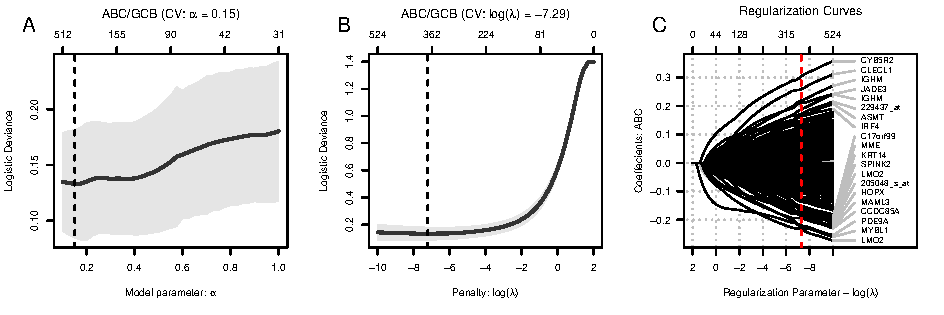
\includegraphics[width=1\textwidth]{figures/figureS1.pdf}
\end{center}
\caption{Ten fold cross validation for the parameters $\alpha$ and $\lambda$ in a logistic regression regularized by elastic net.
In panels A and B the deviance is plotted against the model parameter $\alpha$ and regularization parameter $\lambda$, respectively.
In Panel C the regularization curves are shown.
Black and grey curves represent selected and non-selected probe-sets, respectively.
Positive and negative coefficients indicate that high expression values for the associated gene are related to ABC and GCB, respectively.
The red line indicates the model chosen through $10$ fold cross validation.
The gene symbols for the $20$ probe-sets associated with the largest absolute coefficients in the chosen gene expression predictors are displayed in Panel C.}
\label{fig:crossval}
\end{figure*}

%latex.default(tableS1, file = "tables/tableS1.tex", title = "",     cgroup = names(studies.vec[-5]), rgroup = c("Wright's method",         "One-by-one", "Reference based"), size = "footnotesize",     label = "tab:confusionABCGCBHEMA", caption = caption)%
\begin{table}[!tbp]
{\footnotesize
\caption{Confusion tables for the ABC/GCB classifiers.
The columns represent cohort based normalisation using the ABC/GCB classifier
based on elastic net.
The first part of the table compares Wright's method for ABC/GCB classification
with the elastic net based.
In the second and third part one-by-one and reference based normalisation is
compared to cohort based normalisation using the ABC/GCB classifier based on
elastic net.\label{tab:confusionABCGCBHEMA}} 
\begin{center}
\begin{tabular}{lrrrcrrrcrrrcrrr}
\hline\hline
\multicolumn{1}{l}{\bfseries }&\multicolumn{3}{c}{\bfseries CHEPRETRO}&\multicolumn{1}{c}{\bfseries }&\multicolumn{3}{c}{\bfseries MDFCI}&\multicolumn{1}{c}{\bfseries }&\multicolumn{3}{c}{\bfseries IDRC}&\multicolumn{1}{c}{\bfseries }&\multicolumn{3}{c}{\bfseries LLMPP R-CHOP}\tabularnewline
\cline{2-4} \cline{6-8} \cline{10-12} \cline{14-16}
\multicolumn{1}{l}{}&\multicolumn{1}{c}{ABC}&\multicolumn{1}{c}{NC}&\multicolumn{1}{c}{GCB}&\multicolumn{1}{c}{}&\multicolumn{1}{c}{ABC}&\multicolumn{1}{c}{NC}&\multicolumn{1}{c}{GCB}&\multicolumn{1}{c}{}&\multicolumn{1}{c}{ABC}&\multicolumn{1}{c}{NC}&\multicolumn{1}{c}{GCB}&\multicolumn{1}{c}{}&\multicolumn{1}{c}{ABC}&\multicolumn{1}{c}{NC}&\multicolumn{1}{c}{GCB}\tabularnewline
\hline
{\bfseries Wright's method}&&&&&&&&&&&&&&&\tabularnewline
~~ABC&$38$&$2$&$ 0$&&$28$&$14$&$ 0$&&$174$&$23$&$  1$&&$90$&$ 3$&$  0$\tabularnewline
~~NC&$ 1$&$4$&$ 0$&&$ 1$&$11$&$ 3$&&$  6$&$26$&$ 12$&&$ 6$&$19$&$  8$\tabularnewline
~~GCB&$ 0$&$2$&$42$&&$ 0$&$ 1$&$29$&&$  5$&$31$&$189$&&$ 0$&$ 5$&$102$\tabularnewline
\hline
{\bfseries One-by-one}&&&&&&&&&&&&&&&\tabularnewline
~~ABC&$34$&$0$&$ 0$&&$24$&$ 0$&$ 0$&&$ 95$&$ 0$&$  0$&&$76$&$ 0$&$  0$\tabularnewline
~~NC&$ 5$&$2$&$ 0$&&$ 6$&$ 4$&$ 0$&&$102$&$19$&$  0$&&$20$&$ 6$&$  0$\tabularnewline
~~GCB&$ 0$&$6$&$42$&&$ 0$&$22$&$35$&&$  4$&$67$&$208$&&$ 0$&$21$&$110$\tabularnewline
\hline
{\bfseries Reference based}&&&&&&&&&&&&&&&\tabularnewline
~~ABC&$29$&$6$&$ 0$&&$16$&$ 0$&$ 0$&&$153$&$ 0$&$  0$&&$89$&$22$&$  3$\tabularnewline
~~NC&$ 0$&$1$&$ 4$&&$ 2$&$12$&$ 0$&&$ 32$&$36$&$  0$&&$ 0$&$ 0$&$ 28$\tabularnewline
~~GCB&$ 0$&$0$&$19$&&$ 0$&$ 6$&$25$&&$  0$&$42$&$202$&&$ 0$&$ 0$&$ 61$\tabularnewline
\hline
\end{tabular}\end{center}}

\end{table}

%latex.default(tableS2, file = "tables/tableS2.tex", title = "",     rgroup = flip(studies.vec)[names(subtab)], cgroup = c("One-by-one normalisation",         "Reference based"), size = "small", label = "tab:BAGShemaclass",     caption = caption)%
\begin{table}[!tbp]
{\small
\caption{Confusion tables for the BAGS classifier. One-by-one and reference
based normalisation are shown in the columns and cohort normalisation in the
rows.\label{tab:BAGShemaclass}} 
\begin{center}
\begin{tabular}{lrrrrrrcrrrrrr}
\hline\hline
\multicolumn{1}{l}{\bfseries }&\multicolumn{6}{c}{\bfseries One-by-one normalisation}&\multicolumn{1}{c}{\bfseries }&\multicolumn{6}{c}{\bfseries Reference based}\tabularnewline
\cline{2-7} \cline{9-14}
\multicolumn{1}{l}{}&\multicolumn{1}{c}{N}&\multicolumn{1}{c}{CB}&\multicolumn{1}{c}{CC}&\multicolumn{1}{c}{M}&\multicolumn{1}{c}{PB}&\multicolumn{1}{c}{UC}&\multicolumn{1}{c}{}&\multicolumn{1}{c}{N}&\multicolumn{1}{c}{CB}&\multicolumn{1}{c}{CC}&\multicolumn{1}{c}{M}&\multicolumn{1}{c}{PB}&\multicolumn{1}{c}{UC}\tabularnewline
\hline
{\bfseries CHEPRETRO}&&&&&&&&&&&&&\tabularnewline
~~Naive&$1$&$ 0$&$  0$&$0$&$ 0$&$ 1$&&$ 2$&$ 0$&$  0$&$ 0$&$ 0$&$ 0$\tabularnewline
~~Centroblast&$0$&$18$&$  0$&$0$&$ 0$&$ 0$&&$ 0$&$ 4$&$  4$&$ 0$&$ 0$&$ 1$\tabularnewline
~~Centrocyte&$0$&$10$&$ 11$&$0$&$ 5$&$ 9$&&$ 0$&$ 0$&$ 25$&$ 1$&$ 0$&$ 0$\tabularnewline
~~Memory&$0$&$ 0$&$  0$&$3$&$ 0$&$ 1$&&$ 0$&$ 0$&$  0$&$ 2$&$ 0$&$ 0$\tabularnewline
~~Plasmablast&$0$&$ 0$&$  0$&$0$&$16$&$ 0$&&$ 0$&$ 0$&$  0$&$ 0$&$ 8$&$ 3$\tabularnewline
~~Unclassified&$0$&$ 7$&$  0$&$0$&$ 4$&$ 3$&&$ 0$&$ 0$&$  2$&$ 2$&$ 0$&$ 5$\tabularnewline
\hline
{\bfseries MDFCI}&&&&&&&&&&&&&\tabularnewline
~~Naive&$1$&$ 1$&$  0$&$1$&$ 2$&$ 3$&&$ 3$&$ 0$&$  0$&$ 1$&$ 0$&$ 2$\tabularnewline
~~Centroblast&$0$&$18$&$  0$&$0$&$ 1$&$ 0$&&$ 0$&$ 9$&$  0$&$ 0$&$ 0$&$ 3$\tabularnewline
~~Centrocyte&$0$&$ 7$&$  8$&$2$&$10$&$ 6$&&$ 0$&$ 0$&$ 22$&$ 1$&$ 0$&$ 1$\tabularnewline
~~Memory&$0$&$ 0$&$  0$&$6$&$ 0$&$ 0$&&$ 0$&$ 0$&$  0$&$ 5$&$ 0$&$ 0$\tabularnewline
~~Plasmablast&$0$&$ 0$&$  0$&$0$&$11$&$ 0$&&$ 0$&$ 0$&$  0$&$ 0$&$ 7$&$ 0$\tabularnewline
~~Unclassified&$0$&$ 1$&$  0$&$1$&$ 7$&$ 5$&&$ 1$&$ 0$&$  0$&$ 2$&$ 1$&$ 3$\tabularnewline
\hline
{\bfseries IDRC}&&&&&&&&&&&&&\tabularnewline
~~Naive&$0$&$ 0$&$  3$&$0$&$ 6$&$ 4$&&$12$&$ 0$&$  0$&$ 0$&$ 1$&$ 0$\tabularnewline
~~Centroblast&$0$&$16$&$ 27$&$0$&$27$&$22$&&$ 2$&$62$&$  2$&$ 0$&$ 5$&$12$\tabularnewline
~~Centrocyte&$0$&$ 0$&$140$&$0$&$39$&$18$&&$ 1$&$ 2$&$146$&$ 7$&$ 8$&$18$\tabularnewline
~~Memory&$0$&$ 0$&$  1$&$8$&$20$&$10$&&$ 0$&$ 0$&$  0$&$35$&$ 3$&$ 1$\tabularnewline
~~Plasmablast&$0$&$ 0$&$  1$&$0$&$74$&$ 4$&&$ 0$&$ 0$&$  0$&$ 1$&$76$&$ 1$\tabularnewline
~~Unclassified&$0$&$ 0$&$ 14$&$0$&$44$&$17$&&$ 7$&$ 0$&$  0$&$ 9$&$16$&$38$\tabularnewline
\hline
{\bfseries LLMPP R-CHOP}&&&&&&&&&&&&&\tabularnewline
~~Naive&$1$&$ 2$&$  0$&$0$&$ 5$&$ 6$&&$ 8$&$ 0$&$  0$&$ 1$&$ 0$&$ 1$\tabularnewline
~~Centroblast&$0$&$32$&$  0$&$0$&$ 2$&$ 7$&&$ 0$&$37$&$  1$&$ 0$&$ 0$&$ 1$\tabularnewline
~~Centrocyte&$0$&$ 5$&$ 54$&$0$&$18$&$12$&&$ 0$&$ 1$&$ 66$&$ 1$&$ 1$&$ 4$\tabularnewline
~~Memory&$0$&$ 0$&$  0$&$5$&$13$&$ 4$&&$ 0$&$ 0$&$  0$&$22$&$ 0$&$ 0$\tabularnewline
~~Plasmablast&$0$&$ 0$&$  0$&$0$&$32$&$ 0$&&$ 0$&$ 0$&$  0$&$ 1$&$24$&$ 4$\tabularnewline
~~Unclassified&$0$&$ 2$&$  0$&$0$&$27$&$ 6$&&$ 7$&$ 1$&$  0$&$ 1$&$ 0$&$21$\tabularnewline
\hline
\end{tabular}\end{center}}

\end{table}

%latex.default(tableS3, file = "tables/tableS3.tex", title = "",     rgroup = names(subtab$onebyone), cgroup = flip(studies.vec)[names(subtab$onebyone[[1]])],     size = "small", label = "tab:confusiondrugonebyone", caption = captionS3)%
\begin{table}[!tbp]
\begin{adjustwidth}{-1in}{0in}
{\small
\caption{Confusion tables for the REGS classifiers.
One-by-one normalization are shown in the rows and cohort normalization in the
columns.\label{tab:confusiondrugonebyone}} 
\begin{center}
\begin{tabular}{lrrrcrrrcrrrcrrr}
\hline\hline
\multicolumn{1}{l}{\bfseries }&\multicolumn{3}{c}{\bfseries CHEPRETRO}&\multicolumn{1}{c}{\bfseries }&\multicolumn{3}{c}{\bfseries MDFCI}&\multicolumn{1}{c}{\bfseries }&\multicolumn{3}{c}{\bfseries IDRC}&\multicolumn{1}{c}{\bfseries }&\multicolumn{3}{c}{\bfseries LLMPP R-CHOP}\tabularnewline
\cline{2-4} \cline{6-8} \cline{10-12} \cline{14-16}
\multicolumn{1}{l}{}&\multicolumn{1}{c}{Sen}&\multicolumn{1}{c}{Int}&\multicolumn{1}{c}{Res}&\multicolumn{1}{c}{}&\multicolumn{1}{c}{Sen}&\multicolumn{1}{c}{Int}&\multicolumn{1}{c}{Res}&\multicolumn{1}{c}{}&\multicolumn{1}{c}{Sen}&\multicolumn{1}{c}{Int}&\multicolumn{1}{c}{Res}&\multicolumn{1}{c}{}&\multicolumn{1}{c}{Sen}&\multicolumn{1}{c}{Int}&\multicolumn{1}{c}{Res}\tabularnewline
\hline
{\bfseries Cyclophosphamide}&&&&&&&&&&&&&&&\tabularnewline
~~Sensitive&$40$&$ 1$&$ 0$&&$34$&$ 5$&$ 0$&&$178$&$  0$&$  0$&&$108$&$ 2$&$ 0$\tabularnewline
~~Intermediate&$ 6$&$17$&$ 0$&&$ 0$&$15$&$ 6$&&$114$&$  0$&$  0$&&$  8$&$32$&$ 1$\tabularnewline
~~Resistant&$ 0$&$ 3$&$22$&&$ 0$&$ 1$&$30$&&$203$&$  0$&$  0$&&$  0$&$15$&$67$\tabularnewline
\hline
{\bfseries Doxorubicin}&&&&&&&&&&&&&&&\tabularnewline
~~Sensitive&$30$&$ 0$&$ 0$&&$29$&$ 0$&$ 0$&&$ 25$&$ 86$&$ 39$&&$ 77$&$ 0$&$ 0$\tabularnewline
~~Intermediate&$21$&$ 6$&$ 0$&&$32$&$ 0$&$ 0$&&$  0$&$  6$&$170$&&$ 78$&$ 1$&$ 0$\tabularnewline
~~Resistant&$ 0$&$14$&$18$&&$ 6$&$12$&$12$&&$  0$&$  0$&$169$&&$ 13$&$43$&$21$\tabularnewline
\hline
{\bfseries Vincristine}&&&&&&&&&&&&&&&\tabularnewline
~~Sensitive&$36$&$ 0$&$ 0$&&$33$&$ 0$&$ 0$&&$ 42$&$ 90$&$ 33$&&$ 78$&$ 0$&$ 0$\tabularnewline
~~Intermediate&$ 7$&$ 9$&$ 0$&&$24$&$ 2$&$ 0$&&$  1$&$ 17$&$136$&&$ 59$&$15$&$ 0$\tabularnewline
~~Resistant&$ 1$&$10$&$26$&&$ 1$&$15$&$16$&&$  1$&$  3$&$172$&&$ 11$&$36$&$34$\tabularnewline
\hline
{\bfseries Combined}&&&&&&&&&&&&&&&\tabularnewline
~~Sensitive&$32$&$ 0$&$ 0$&&$33$&$ 0$&$ 0$&&$135$&$ 14$&$  1$&&$ 87$&$ 0$&$ 0$\tabularnewline
~~Intermediate&$19$&$ 9$&$ 0$&&$27$&$ 1$&$ 0$&&$ 19$&$143$&$ 21$&&$ 70$&$ 0$&$ 0$\tabularnewline
~~Resistant&$ 0$&$13$&$16$&&$ 3$&$13$&$14$&&$  0$&$ 27$&$135$&&$ 16$&$42$&$18$\tabularnewline
\hline
\end{tabular}\end{center}}
\end{adjustwidth}
\end{table}

%latex.default(tableS4, file = "tables/tableS4.tex", title = "",     rgroup = names(subtab$refbased), cgroup = flip(studies.vec)[names(subtab$refbased[[1]])],     size = "small", label = "tab:confusiondrugreference", caption = captionS4)%
\begin{table}[!tbp]
{\small
\caption{Confusion tables for the REGS classifiers.
Reference based normalisation are shown in the rows and cohort normalisation in
the columns. Note, 30 samples were used as reference data and hence not present
in this table.\label{tab:confusiondrugreference}} 
\begin{center}
\begin{tabular}{lrrrcrrrcrrrcrrr}
\hline\hline
\multicolumn{1}{l}{\bfseries }&\multicolumn{3}{c}{\bfseries CHEPRETRO}&\multicolumn{1}{c}{\bfseries }&\multicolumn{3}{c}{\bfseries MDFCI}&\multicolumn{1}{c}{\bfseries }&\multicolumn{3}{c}{\bfseries IDRC}&\multicolumn{1}{c}{\bfseries }&\multicolumn{3}{c}{\bfseries LLMPP R-CHOP}\tabularnewline
\cline{2-4} \cline{6-8} \cline{10-12} \cline{14-16}
\multicolumn{1}{l}{}&\multicolumn{1}{c}{Sen}&\multicolumn{1}{c}{Int}&\multicolumn{1}{c}{Res}&\multicolumn{1}{c}{}&\multicolumn{1}{c}{Sen}&\multicolumn{1}{c}{Int}&\multicolumn{1}{c}{Res}&\multicolumn{1}{c}{}&\multicolumn{1}{c}{Sen}&\multicolumn{1}{c}{Int}&\multicolumn{1}{c}{Res}&\multicolumn{1}{c}{}&\multicolumn{1}{c}{Sen}&\multicolumn{1}{c}{Int}&\multicolumn{1}{c}{Res}\tabularnewline
\hline
{\bfseries Cyclophosphamide}&&&&&&&&&&&&&&&\tabularnewline
~~Sensitive&$13$&$10$&$ 0$&&$26$&$ 4$&$ 0$&&$134$&$ 32$&$  0$&&$89$&$ 5$&$ 0$\tabularnewline
~~Intermediate&$ 0$&$ 7$&$10$&&$ 0$&$10$&$ 1$&&$  3$&$ 77$&$ 29$&&$ 0$&$27$&$ 9$\tabularnewline
~~Resistant&$ 0$&$ 0$&$19$&&$ 0$&$ 0$&$20$&&$  0$&$  9$&$181$&&$ 0$&$ 2$&$71$\tabularnewline
\hline
{\bfseries Doxorubicin}&&&&&&&&&&&&&&&\tabularnewline
~~Sensitive&$18$&$ 2$&$ 0$&&$19$&$ 0$&$ 0$&&$132$&$  7$&$  0$&&$50$&$15$&$ 0$\tabularnewline
~~Intermediate&$ 0$&$14$&$ 2$&&$ 0$&$21$&$ 0$&&$ 24$&$143$&$  3$&&$ 0$&$55$&$13$\tabularnewline
~~Resistant&$ 0$&$ 0$&$23$&&$ 0$&$ 3$&$18$&&$  0$&$ 16$&$140$&&$ 0$&$ 0$&$70$\tabularnewline
\hline
{\bfseries Vincristine}&&&&&&&&&&&&&&&\tabularnewline
~~Sensitive&$18$&$ 5$&$ 0$&&$16$&$ 6$&$ 0$&&$127$&$ 32$&$  0$&&$71$&$ 0$&$ 0$\tabularnewline
~~Intermediate&$ 0$&$10$&$ 1$&&$ 0$&$ 8$&$ 9$&&$ 12$&$ 83$&$ 46$&&$ 9$&$49$&$ 0$\tabularnewline
~~Resistant&$ 0$&$ 0$&$25$&&$ 0$&$ 0$&$22$&&$  1$&$ 10$&$154$&&$ 0$&$10$&$64$\tabularnewline
\hline
{\bfseries Combined}&&&&&&&&&&&&&&&\tabularnewline
~~Sensitive&$19$&$ 3$&$ 0$&&$23$&$ 1$&$ 0$&&$125$&$ 14$&$  0$&&$64$&$12$&$ 0$\tabularnewline
~~Intermediate&$ 0$&$11$&$ 5$&&$ 0$&$16$&$ 0$&&$ 12$&$148$&$ 14$&&$ 0$&$46$&$10$\tabularnewline
~~Resistant&$ 0$&$ 0$&$21$&&$ 0$&$ 0$&$21$&&$  0$&$  6$&$146$&&$ 0$&$ 0$&$71$\tabularnewline
\hline
\end{tabular}\end{center}}

\end{table}

\clearpage



\section{Graham's formula}
\label{sec:graham}
This section derives Graham's formula which, in our context, yields the posterior probability of being sensitive to the combination of two drugs, given sensitivity to the individual drugs.
For simplicity, the formula is derived for two drugs.
The formula straightforwardly generalizes to three or more drugs.

Let $C$, $H$, and $B$ be Bernoulli distributed random variables with probability parameter $1/2$, where
$C = 1$ indicates sensitivity to Cyclophosphamide $C$,
$H = 1$ indicates sensitivity to Doxorubicin $H$, and
$B = 1$ indicates sensitivity to the combination of $H$ and $C$.
Conversely, $C,H,$ and $B = 0$ indicates resistance towards $C,H,$ and $B$, respectively.
Under an assumption of conditional drug independence
\begin{align*}
  P(C=1, H=1| B=1) &= P(C=1 | B=1) P(H=1 | B=1), \text{ and } \\
  P(C=1, H=1| B=0) &= P(C=1 | B=0) P(H=1 | B=0)
\end{align*}
we have that
\begin{align*}
  &P(B=1 | H=1, C=1)
  \\&\qquad
   = \frac{P(C=1, H=1, B=1)}
          {P(C=1, H=1)}
  \\&\qquad
   = \frac{P(C=1, H=1 | B=1) P(B=1)}
          {P(C=1, H=1, B=1) + P(C=1, H=1, B=0)}
  \\&\qquad
   = \frac{P(C=1 | B=1) P(H=1 | B=1) P(B=1)}
          {P(C=1, H=1 | B=1) P(B=1) + P(H=1, C=1| B=0) P(B=0)},
\end{align*}
by the definition of conditional probabilities, the law of total probability, and the assumptions.
From the distributional assumption on $B$, $P(B=0) = P(B=1) = 1/2$, and the above then simplifies to:
\begin{equation*}
  P(B=1 | H=1, C=1)
   = \frac{P(C=1 | B=1) P(H=1 | B=1)}
          {P(C=1, H=1 | B=1) + P(H=1, C=1 | B=0)}.
\end{equation*}
For notational convenience, we abbreviate
$p_C = P(C=1 | B=1)$,
$p_H = P(H=1 | B=1)$,
$p_{CH} = P(B=1 | H=1, C=1)$.
The distributional assumptions then imply:
\begin{align*}
  p_{CH}
  &= \frac{p_C p_H}
          {p_C p_H + P(C=1 | B=0) P(H=1 | B=0)}
  \\
  &= \frac{p_C p_H}
          {p_C p_H + P(B=0 | C=1) P(B=0 | H=1)}
  \\
  &= \frac{p_C p_H}
          {p_C p_H + \bigl(1 - P(B=1 | C=1)\bigr)\bigl(1 - P(B=1 | H=1)\bigr)}
  \\
  &= \frac{p_C p_H}
          {p_C p_H + (1 - p_C)(1 - p_H)},
\end{align*}
which is the two-drug equivalent to the used formula.




\section{RMA normalization}
Recall that ordinary robust multichip average (RMA) pre-processing consists of three steps: (1) Background adjustment, (2) quantile normalization, and (3) summarization of probes to probe-sets, see e.g.\ \citep{Irizarry2003, Irizarry2003b}. For completeness we review ordinary cohort based RMA normalization.

\subsection{Backgroud correction}
In order to produce background adjusted probe intensities we will use the within array normal-exponential de-convolution scheme as implemented by the \texttt{rma.background.correct} command in the Bioconductor package \texttt{preprocessCores}, see
\citep{Irizarry2003b,Bolstad2004}.


\subsection{Quantile normalization}
Let $x_{ijk}$ be the $\log_2$-transformed and background adjusted cohort data, where $i = 1,\dots,I$ index the arrays of the cohort data, $j=1,\dots,J$  index the probe-sets, and $k=1,\dots,K_j$ index the probes nested within probe-sets.

Furthermore, let $G_i$ denote the empirical cumulative distribution function (ECDF) of the probes $\{x_{ijk}\}_{jk}$ on the $i$'th cohort array and $F$ the ECDF of the across array averaged sample quantiles $\{\bar{x}_{\cdot (jk)}\}_{ij}$, where $\{x_{i(jk)}\}_{jk}$ is the order statistic of all probes on the $i$'th cohorte array based on the lexicographic ordering of the indices $\{jk\}$. Then each data point is quantile normalized in the following way
\begin{equation*}
     \tilde{x}_{ijk} = F^{-1}(G_i(x_{ijk})),
\end{equation*}
where $F^{-1}$ is calculated as the quantiles of type 2 \citep{Hyndman1996}.
This step is performed by the \texttt{RMA\_norm} function with option \texttt{generateQuan} equal to one in the \hemaClass{} package.

\subsection{Summarisation}

For each probe-set $j$ we let $\mu_{ij}$ represent the $\log_2$-scale expression level for array $i$ and probeset $j$, $\alpha_{jk}$ the probe affinity effect, and the $\epsilon_{ijk}$'s are independent identically distributed  error terms with mean 0 and formulate the following linear additive model
\begin{equation*}
   \tilde{x}_{ijk} = \mu_{ij} + \alpha_{jk}+ \epsilon_{ijk},
\end{equation*}
where $\sum_{k=0}^{n_j} \alpha_{jk} = 0$ for all probe-sets. The parameters are estimated by median polish \citep{Holder2001}. The probe affinity estimates are denoted by $\hat{\alpha}_{jk}$.

The RMA normalized cohort data are then given by
\begin{equation*}
   \hat{x}_{ij\cdot} = \hat{\mu}_{ij},
\end{equation*}
where the dot notation indicate the mean across the index.
This step is performed by the \texttt{RMA\_sum} function in the \hemaClass{} package.




\section{One-by-one RMA normalization of user supplied data}
\subsection{Backgroud correction}

The background correction in one-by-one RMA normalization is unaltered as it is already works in an one-by-one fashion.


\subsection{Quantile normalization}

Let $x_{ijk}$ be the $\log_2$-transformed and background corrected reference data, where $i = 1,\dots,I_R$ index the arrays of the reference data, $j=1,\dots,J$  index the probe-sets, and $k=1,\dots,K_j$ index the probes. Assume $x_{ijk}$ has been RMA normalized as described above. Similarly,  let $y_{ijk}$ be the log2-transformed and background corrected user supplied data, where $i = 1,\dots,I_U$ index the arrays of the user supplied data, $j=1,\dots,J$  index the probe-sets, and $k=1,\dots,K_j$ index the probes.

Furthermore, let $H_i$ denote the ECDF of the user supplied data $\{y_{ijk}\}_{jk}$, respectively.

As quantile normalizer the ECDF of the background corrected reference data is used in place of the ususally applied ECDF of the mean of the sample quantiles
\begin{equation*}
   \tilde{y}_{ijk} = F^{-1}(H_i(y_{ijk})).
\end{equation*}
This step is performed by the \texttt{RMA\_norm} function with options \texttt{generateQuan} equal to zero and \texttt{quantile} equal to the quantiles of the reference data in the \hemaClass{} package.


\subsection{Summarization}

To mimic the RMA summarization the probe effects estimated by median polish on the reference data is subtracted all probes of the user data
\begin{equation*}
   \hat{y}_{ijk} = \tilde{y}_{ijk} - \hat{\alpha}_{jk},
\end{equation*}
in place of the usual estimated probe effects from the cohort.
The pre-processed expression value for each probe-set is then estimated as the median of the associated probes.
\begin{equation*}
   \hat{y}_{ij\cdot} = \median_{k \in \{1,\dots,n_j \}} \{ \hat{y}_{ijk} \}.
\end{equation*}


\section{Classification}
To ensure identical classification probabilities whether data is supplied as a cohort or one-by-one, we finally subtract the median of each probe-set in the reference from the corresponding probe-set and scale by the standard deviation of each probe-set in the reference data
\begin{equation*}
  (\hat{y}_{ij\cdot} - \hat{x}_{\cdot j\cdot})/s_{\cdot j\cdot},
\end{equation*}
where
$\hat{x}_{\cdot j\cdot} = \median_{i \in \{1,\dots,I_R \}} \{\hat{x}_{ij\cdot}\}$ and $s_{\cdot j\cdot} = \std_{i \in \{1,\dots,I_R\}} \{\hat{x}_{ij\cdot}\}$.


% \end{document}